\chapter{Ausblick}

Sowohl durch den Industriepartner als auch durch das Team selbst kamen verschiedene Ideen für weitergehende Features auf. Aus Zeitgründen konnten leider nicht alle Ideen umgesetzt werden.

\section{'Workflow'}

Ein Wunsch der Industriepartner war es, den momentanen Arbeitsablauf abbilden zu können


\xxx[ Workflow-Feature ]

\begin{figure}[H]
	\centering
	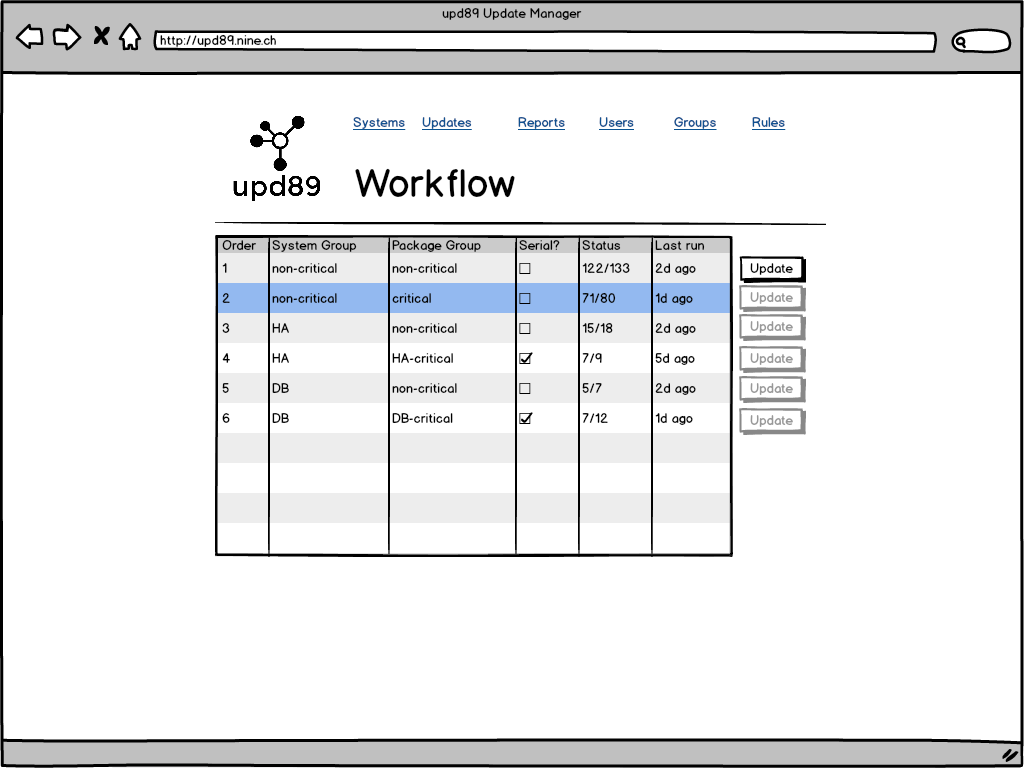
\includegraphics[width=\linewidth]{files/mockups/workflow}
	\caption{Konzept Workflow-Feature}
	\label{fig:ausblick:workflow}
\end{figure}

\begin{figure}[H]
	\centering
	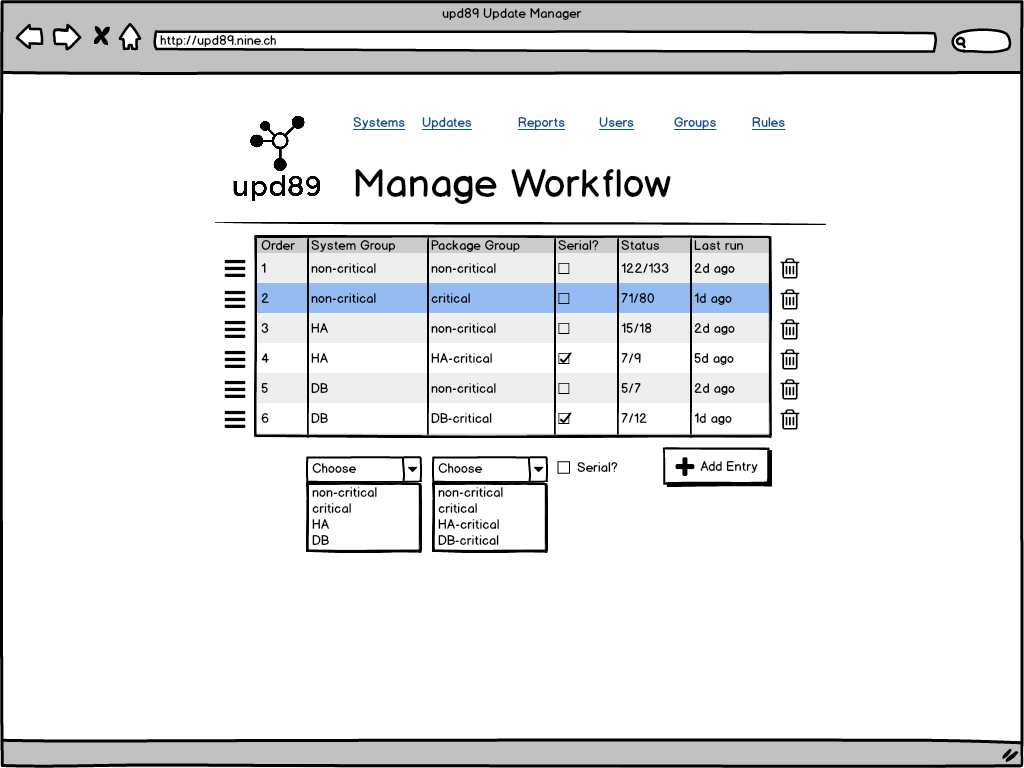
\includegraphics[width=\linewidth]{files/mockups/workflow_CRUD}
	\caption{Konzept Workflow-Feature bearbeiten}
	\label{fig:ausblick:workflow_crud}
\end{figure}

\xxx[ Separater API-Endpunkt für einfachere Registrierung ]

\xxx[ Dry-Run ]

\xxx[ Message-Queue, z.B. RabbitMQ ]

